

\begin{table*}[htbp]
\centering
\small
\caption{WikiText2 perplexity with 2048 sequence length. The lower is the better.}
\scalebox{0.9}{
\begin{tabular}{llcccccccccc}
\toprule
  \multicolumn{2}{c}{WikiText2 Perplexity ↓} 
& Llama-3
& \multicolumn{3}{c}{Llama-2} 
& \multicolumn{3}{c}{Llama} 
& Mistral & Mixtral & Yi \\
\cmidrule{1-9}
  Precision         & Algorithm  
& 8B      
&   7B    &   13B   &   70B   
&   7B    &   13B   &   30B   
&   7B    &   8x7B  &   34B \\
\midrule
\texttt{FP16}       & - 
&  6.14   
&  5.47   &  4.88   &  3.32   
&  5.68   &  5.09   &  4.10   
&  5.25   &  3.84   &  4.60 \\
\midrule
\texttt{W8A8}       & SmoothQuant 
&  6.28   
&  5.54   &  4.95   &  3.36 
&  5.73   &  5.13   &  4.23   
&  5.29   &  3.89   &  4.69 \\
\midrule
\multirow{2}{*}{\makecell[l]{\texttt{W4A16} \\ g128}} & GPTQ-R 
&  6.56   
&  5.63   &  4.99   &  3.43
&  5.83   &  5.20   &  4.22   
&  5.39   &  4.08   &  4.68 \\
                    & AWQ 
&  6.54   
&  5.60   &  4.97   &  3.41
&  5.78   &  5.19   &  4.21   
&  5.37   &  4.02   &  4.67 \\
\midrule
\multirow{2}{*}{\texttt{W4A4}} & \multirow{2}{*}{QuaRot}
&  \textcolor{gray}{8.20}
&  \textcolor{gray}{6.10}   &  \textcolor{gray}{5.40}   &  \textcolor{gray}{3.79}
&  \textcolor{gray}{6.26}   &  \textcolor{gray}{5.55}   &  \textcolor{gray}{4.60}   
&  \textcolor{gray}{5.71}   &  \textcolor{gray}{NaN}    &  \textcolor{gray}{NaN} \\
              &  
&  8.33   
&  6.19   &  5.45   &  3.83
&  6.34   &  5.58   &  4.64   
&  5.77   &  NaN    &  NaN \\
\midrule
\multirow{4}{*}{\makecell[l]{\texttt{W4A4} \\ g128}} & \multirow{2}{*}{QuaRot}$\dagger$
&  \textcolor{gray}{7.32}
&  \textcolor{gray}{5.93}   &  \textcolor{gray}{5.26}   &  \textcolor{gray}{3.61}
&  \textcolor{gray}{6.06}   &  \textcolor{gray}{5.40}   &  \textcolor{gray}{4.44}   
&  \textcolor{gray}{5.54}   &  \textcolor{gray}{NaN}    &  \textcolor{gray}{NaN} \\
              &  
&  7.51   
&  6.00   &  5.31   &  3.64
&  6.13   &  5.43   &  4.48   
&  5.58   &  NaN    &  NaN \\
\cmidrule{2-12}
& \multirow{2}{*}{Atom}$\dagger$
&  \textcolor{gray}{7.57}
&  \textcolor{gray}{6.03}   &  \textcolor{gray}{5.27}   &  \textcolor{gray}{3.69}
&  \textcolor{gray}{6.16}   &  \textcolor{gray}{5.46}   &  \textcolor{gray}{4.55}   
&  \textcolor{gray}{5.66}   &  \textcolor{gray}{4.42}    &  \textcolor{gray}{4.92} \\
              &  
&  7.76   
&  6.12   &  5.31   &  3.73 
&  6.25   &  5.52   &  4.61   
&  5.76   &  4.48   &  4.97 \\
\arrayrulecolor{black}
\midrule
\multirow{3}{*}{\texttt{W4A8KV4}} & RTN
&  9.50   
&  6.51   &  5.40   &  3.90 
&  6.51   &  5.71   &  4.91   
&  6.18   &  5.02   &  6.52 \\
                    & AWQ
&  7.90   
&  6.28   &  5.25   &  3.68
&  6.33   &  5.59   &  4.61   
&  5.92   &  4.58   &  5.26 \\
                    & \cellcolor{mylightblue}\algo
& \cellcolor{mylightblue}\textbf{6.81}
&  \cellcolor{mylightblue}\textbf{5.75}   &  \cellcolor{mylightblue}\textbf{5.11}   & \cellcolor{mylightblue}\textbf{3.50}
&  \cellcolor{mylightblue}\textbf{5.92}   &  \cellcolor{mylightblue}\textbf{5.27}   & \cellcolor{mylightblue}\textbf{4.31}   
&  \cellcolor{mylightblue}\textbf{5.44}   &  \cellcolor{mylightblue}\textbf{4.17}   & \cellcolor{mylightblue}\textbf{4.73} \\
\midrule
\multirow{3}{*}{\makecell[l]{\texttt{W4A8KV4} \\ g128}} & RTN
&  7.25   
&  5.99   &  5.19   &  3.70
&  6.23   &  5.46   &  4.56   
&  5.59   &  4.39   &  5.49 \\
                    & AWQ
&  6.94   
&  5.83   &  5.12   &  3.51
&  5.93   &  5.36   &  4.39   
&  5.50   &  4.23   &  4.78 \\
                    & \cellcolor{mylightblue}\algo
& \cellcolor{mylightblue}\textbf{6.70}
& \cellcolor{mylightblue}\textbf{5.67} & \cellcolor{mylightblue}\textbf{5.06} & \cellcolor{mylightblue}\textbf{3.46}
& \cellcolor{mylightblue}\textbf{5.88} & \cellcolor{mylightblue}\textbf{5.23} & \cellcolor{mylightblue}\textbf{4.27}   
& \cellcolor{mylightblue}\textbf{5.41}          & \cellcolor{mylightblue}\textbf{4.13} & \cellcolor{mylightblue}\textbf{4.73}\\
\bottomrule
\multicolumn{11}{l}{* Grayed results use Wikitext2 as calibaration dataset.} \\
\multicolumn{11}{l}{$\dagger$ QuaRot and Atom apply group quantization to activations as well.} \\

\end{tabular}
}
\label{tab:evaluation:wikitext}
\end{table*}


\begin{table*}[t]
\centering
\small
\caption{Zero-shot accuracy on five common sense tasks with 2048 sequence length.}
\scalebox{0.98}{
\begin{tabular}{lllcccccc}
\toprule
\multirow{2}{*}{Llama-2} 
& \multirow{2}{*}{Precision} 
& \multirow{2}{*}{Method}
& \multicolumn{6}{c}{Zero-shot Accuracy ↑} \\ \cmidrule{4-9}
& 
& 
& PQ & ARC-e & ARC-c & HS & WG & Avg. \\ \midrule
 & \texttt{FP16} 
 & -      
 & 79.05 & 74.58 & 46.25 & 76.05 & 68.98 & 68.98
 \\ \cmidrule{2-9}
 & \texttt{W4A4} 
 & Quarot 
 & 76.77 & 69.87 & 40.87 & 72.16 & 63.77 & 64.69
 \\ 
 \cmidrule{2-9}
 7B 
 & \texttt{W4A4} g128
 & Atom 
 & 75.14 & 52.99 & 38.40 & 69.37 & 62.75 & 59.73
 \\ \cmidrule{2-9}
 & \texttt{W4A8KV4} 
 & \cellcolor{mylightblue}\algo 
 & \cellcolor{mylightblue}78.07 & \cellcolor{mylightblue}73.11 & \cellcolor{mylightblue}45.05 & \cellcolor{mylightblue}74.12 & \cellcolor{mylightblue}67.48 & \cellcolor{mylightblue}67.57
 \\ 
 & \makecell[l]{\texttt{W4A8KV4} g128}
 & \cellcolor{mylightblue}\algo
 & \cellcolor{mylightblue}\textbf{78.07} & \cellcolor{mylightblue}\textbf{73.32} & \cellcolor{mylightblue}\textbf{44.80} & \cellcolor{mylightblue}\textbf{74.98} & \cellcolor{mylightblue}\textbf{68.59} & \cellcolor{mylightblue}\textbf{67.95}
 \\ \midrule
 & \texttt{FP16} 
 & -      
 & 80.52 & 77.44 & 49.06 & 79.38 & 72.22 & 71.72
 \\ \cmidrule{2-9}
 & \texttt{W4A4} 
 & Quarot 
 & 78.89 & 72.98 & 46.59 & 76.37 & 70.24 & 69.01
 \\
 \cmidrule{2-9}
 13B 
 & \texttt{W4A4} g128
 & Atom 
 & 76.50 & 57.49 & 42.32 & 73.84 & 67.40 & 63.51
 \\ \cmidrule{2-9}
 & \texttt{W4A8KV4} 
 & \cellcolor{mylightblue}\algo
 & \cellcolor{mylightblue}\textbf{79.71}  & \cellcolor{mylightblue}75.97 & \cellcolor{mylightblue}48.38 & \cellcolor{mylightblue}77.80 & \cellcolor{mylightblue}\textbf{70.96} & \cellcolor{mylightblue}70.56
 \\ 
 & \makecell[l]{\texttt{W4A8KV4} g128}
 & \cellcolor{mylightblue}\algo
 & \cellcolor{mylightblue}79.43  & \cellcolor{mylightblue}\textbf{77.06} & \cellcolor{mylightblue}\textbf{48.81} & \cellcolor{mylightblue}\textbf{78.35} & \cellcolor{mylightblue}70.48 & \cellcolor{mylightblue}\textbf{70.83}
 \\\midrule
 & \texttt{FP16} 
 & -      
 & 82.70 & 81.02 & 57.34 & 83.82 & 77.98 & 76.57
 \\ \cmidrule{2-9}
 & \texttt{W4A4} 
 & Quarot 
 & 82.43 & 80.43 & 56.23 & 81.82 & 76.24 & 75.43
 \\
 \cmidrule{2-9}
 70B
 & \texttt{W4A4} g128
 & Atom 
 & 79.92 & 58.25 & 46.08 & 79.06 & 74.27 & 67.52
 \\ \cmidrule{2-9}
 & \texttt{W4A8KV4} 
 & \cellcolor{mylightblue}\algo
 & \cellcolor{mylightblue}82.64  & \cellcolor{mylightblue}79.80 & \cellcolor{mylightblue}\textbf{56.83}  & \cellcolor{mylightblue}82.78  & \cellcolor{mylightblue}77.51  & \cellcolor{mylightblue}75.91 
 \\ 
 & \makecell[l]{\texttt{W4A8KV4} g128}
 & \cellcolor{mylightblue}\algo
 & \cellcolor{mylightblue}\textbf{82.92}  & \cellcolor{mylightblue}\textbf{80.93} & \cellcolor{mylightblue}56.40 & \cellcolor{mylightblue}\textbf{83.28} & \cellcolor{mylightblue}\textbf{78.45} & \cellcolor{mylightblue}\textbf{76.40}
 \\
 \bottomrule
 \multicolumn{9}{l}{* For reference, using MX-FP4 for \texttt{W4A4} quantizing Llama-7B model will decrease the }\\
 \multicolumn{9}{l}{  accuracy from 72.9 to 63.7 on ARC easy and from 44.7 to 35.5 on ARC challenge task.~\cite{rouhani2023microscaling}}
\end{tabular}
}
\label{tab:evaluation:zero-shot}
\end{table*}


\begin{figure*}[t]
    \centering
    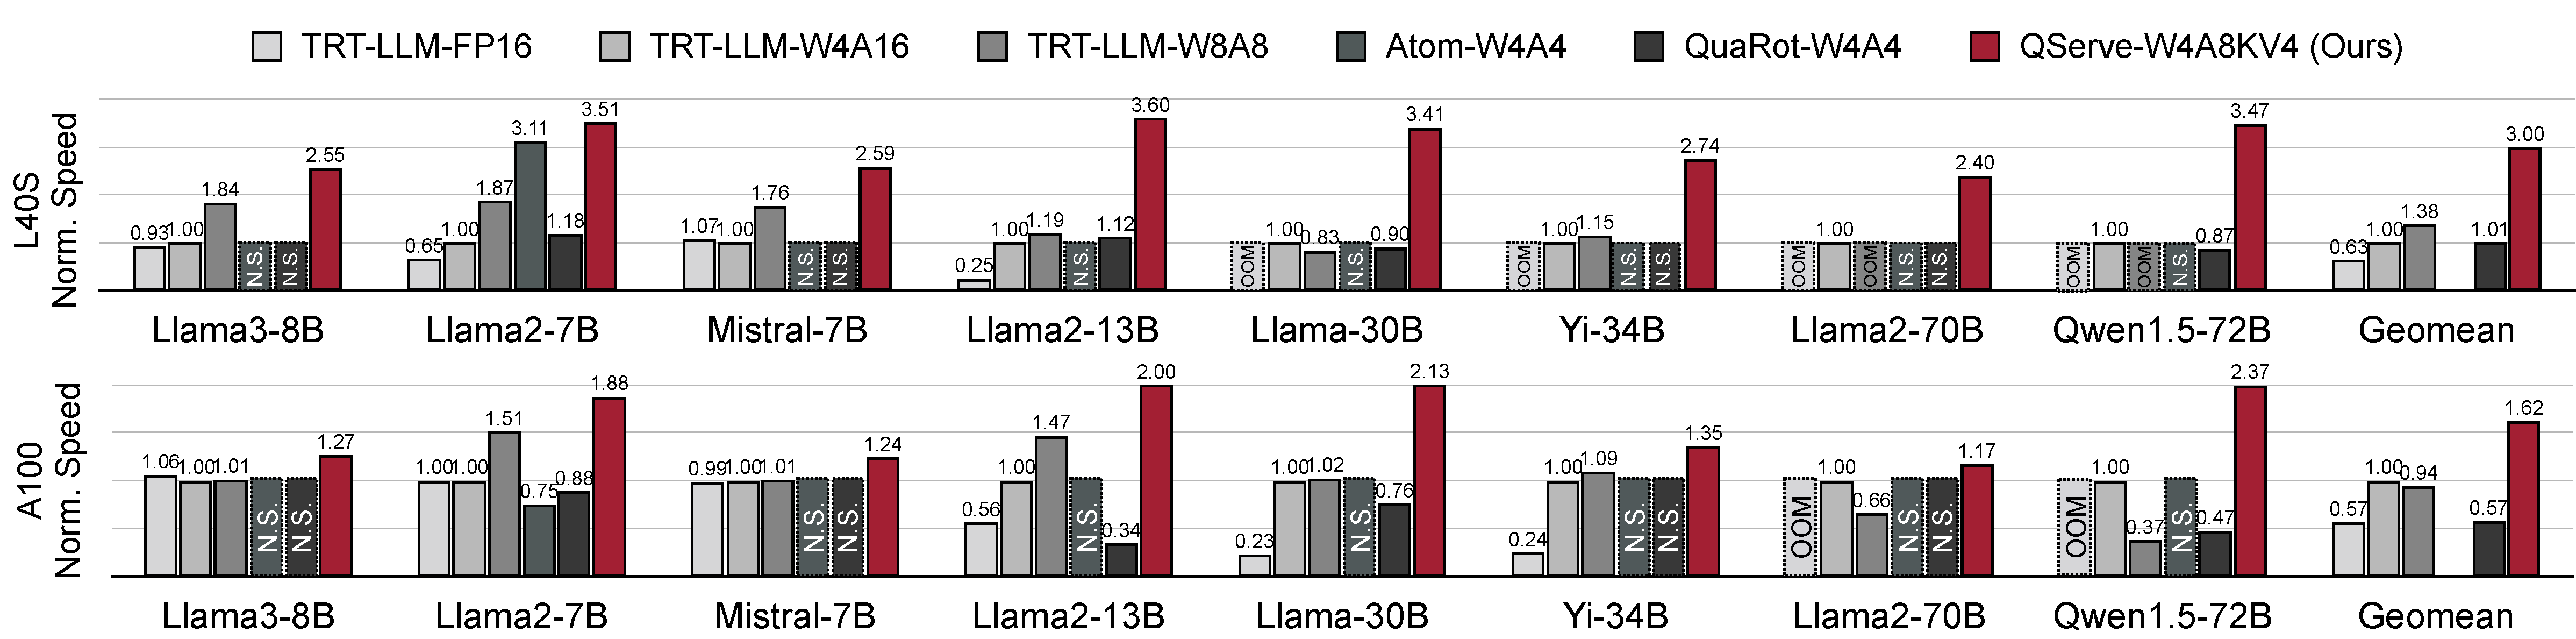
\includegraphics[width=\linewidth]{figure/6-evaluation/main_speed.pdf}
    \caption{\system significantly outperforms existing large language model (LLM) serving frameworks in batched generation tasks across different LLMs, ranging from 7B to 72B models. It achieves an average speedup of 2.36$\times$ over the state-of-the-art LLM serving system, TensorRT-LLM v0.9.0, on the L40S GPU, and it is also 1.68$\times$ faster on the  A100 GPU. All experiments were conducted under the same device memory budget (\ie 80GB on A100 and 48GB on L40S). We omit the geometric mean speedup of Atom since it only supports Llama2-7B. For absolute values, see Table \ref{tab:abs_main_speed}.}%
    \label{fig:evaluation:main_speed}
\end{figure*}


\begin{table*}[ht]
\centering
\small
\caption{The absolute token generation throughput of \system and TensorRT-LLM in Fig. \ref{fig:evaluation:main_speed}. \textsuperscript{*}: we calculate the speedup over highest achieveable throughput from TensorRT-LLM across all three precision configurations. Our \system system achieves competitive throughput on L40S GPU compared to TensorRT-LLM on A100, effectively reducing the dollar cost of LLM serving by 3$\times$. Unit: tokens/second.}
\scalebox{0.98}{\begin{tabular}{cccccccccc}
\toprule
\multirow{2}{*}{Device} & \multirow{2}{*}{System} & Llama-3 & Llama-2 & Mistral & LLama-2 & LLaMA & Yi & Llama-2 & Qwen1.5 \\
 & & 8B & 7B & 7B & 13B & 30B & 34B & 70B & 72B \\
\midrule

& TRT-LLM-\texttt{FP16} & 1326 & 444 & 1566 & 92 & OOM & OOM & OOM & OOM
\\ \cmidrule{2-10}
& TRT-LLM-\texttt{W4A16} & 1431 & 681 & 1457 & 368 & 148 & 313 & 119 & 17

\\ \cmidrule{2-10}
L40S & TRT-LLM-\texttt{W8A8} & 2634 & 1271 & 2569 & 440 & 123 & 364 & OOM & OOM
\\ \cmidrule{2-10}
 & QServe (Ours) 
 & \textbf{3656} & \textbf{2394} & \textbf{3774} & \textbf{1327} & \textbf{504} & \textbf{869} & \textbf{286} & \textbf{59} 
  \\ \cmidrule{2-10}
 & Speedup\textsuperscript{*} & \textbf{1.39$\times$} & \textbf{1.88$\times$} & \textbf{1.47}$\times$ & \textbf{3.02}$\times$ & \textbf{3.41}$\times$ & \textbf{2.39}$\times$ & \textbf{2.40}$\times$ & \textbf{3.47}$\times$ 
 \\\midrule


& TRT-LLM-\texttt{FP16} & 2503 & 1549 & 2371 & 488 & 80 & 145 & OOM & OOM 
\\ \cmidrule{2-10}

& TRT-LLM-\texttt{W4A16} & 2370 & 1549 & 2403 & 871 & 352 & 569 & 358 & 143 

\\ \cmidrule{2-10}
A100 & TRT-LLM-\texttt{W8A8} & 2396 & 2334 & 2427 & 1277 & 361 & 649 & 234 & 53
 \\ \cmidrule{2-10}
 & QServe (Ours) 
 & \textbf{3005} & \textbf{2908} & \textbf{2970} & \textbf{1741} & \textbf{749} & \textbf{797} & \textbf{419} & \textbf{340}
 \\
 \cmidrule{2-10}
 & Speedup\textsuperscript{*} & \textbf{1.20}$\times$ & \textbf{1.25}$\times$ & \textbf{1.22}$\times$ & \textbf{1.36}$\times$ & \textbf{2.07}$\times$ & \textbf{1.23}$\times$ & \textbf{1.17}$\times$ & \textbf{2.38}$\times$ 
 \\ 
 

 \bottomrule
\end{tabular}
}
\label{tab:abs_main_speed}
\vspace{-10pt}
\end{table*}


\vspace{-5pt}
\section{Evaluation}
\label{sect:evaluation}

\subsection{Evaluation Setup}

\textbf{Algorithm.} The \algo quantization algorithm is implemented using HuggingFace~\cite{transformers} on top of PyTorch~\cite{pytorch}. We use per-token symmetric INT8 quantization on activations, and per-head asymmetric INT4 quantization on KV cache. 
``\textbf{\texttt{W4A8KV4}} g128" refers to the case where \system used progressive group quantization on weights: per-channel symmetric INT8 quantization followed by asymmetric INT4 quantization with a group size of 128, while ``\textbf{\texttt{W4A8KV4}}" is the per-channel counterpart for weight quantization. %

\textbf{System.} \system serving system is implemented using CUDA and PTX assembly for high-performance GPU kernels. We also provide a purely PyTorch-based front-end framework for better flexibility. 
For the throughput benchmarking, we perform all experiments under PyTorch 2.2.0 with CUDA 12.2, unless otherwise specified. The throughput numbers reported are real measurements on NVIDIA GPUs. For baseline systems, we use TensorRT-LLM v0.9.0 and latest main branches from QuaRot and Atom as of April 18\textsuperscript{th}, 2024. Paged attention is enabled for all systems except QuaRot, which does not offer corresponding support.

\subsection{Accuracy Evaluation}


\paragraph{Benchmarks.}
We evaluated \algo on the Llama-1~\cite{touvron2023llama}, Llama-2~\cite{touvron2023llama2}, Llama-3 families, Mistral-7B~\cite{jiang2023mistral}, Mixtral-8x7B~\cite{jiang2024mixtral} and Yi-34B~\cite{ai2024yi} models. Following previous literature~\cite{llmint8,gptq,zhao2023atom,ashkboos2024quarot, xiao2023smoothquant,lin2023awq}, we evaluated \algo-quantized models on language modeling and zero-shot tasks. Specifically, we evaluated on WikiText2~\cite{wikitext} for perplexity, and evaluated on PIQA~\cite{piqa} (PQ), ARC~\cite{arc}, HellaSwag~\cite{hellaswag} (HS) and WinoGrande~\cite{sakaguchi2019winogrande} (WG) with \texttt{lm\_eval}~\cite{eval-harness}.

\paragraph{Baselines.}
We compared \algo to widely used post-training LLM quantization techiniques, SmoothQuant~\cite{xiao2023smoothquant}, GPTQ~\cite{gptq}, AWQ~\cite{lin2023awq}, and recently released state-of-the-art 4-bit weight-activation quantization frameworks, Atom~\cite{zhao2023atom} and QuaRot~\cite{ashkboos2024quarot}. For SmoothQuant, we uses static per-tensor symmetric 8-bit quantization for KV cache following the settings in the TensorRT-LLM~\cite{trtllm}.
For GPTQ, we use their latest version with ``reorder" trick, denoted as ``GPTQ-R". For QuaRot and Atom, we mainly evaluated using Pile validation dataset as calibration dataset. We also report their results with WikiText2 as calibration dataset in gray color. For ``\textbf{\texttt{W4A8KV4}} g128" setting, both QuaRot and Atom does not support progressive group quantization, and thus we evaluated them using ordinary group weight quantization (\ie, each group has one FP16 scale factor). Unsupported models and quantization settings will be reported as NaN.




\paragraph{WikiText2 perplexity.}\tab{tab:evaluation:wikitext} compares the Wikitext2 perplexity results between \algo and other baselines. For Llama-2-7B, compared to \textbf{\texttt{W8A8}} SmoothQuant and \textbf{\texttt{W4A16}} AWQ, \algo only increased perplexity by up to 0.16 %
\algo consistently outperformed Atom with either \textbf{\texttt{W4A4}} or \textbf{\texttt{W4A8KV4}} quantization precision. \algo also showed up to 0.49 perplexity improvement compared to \textbf{\texttt{W4A4}} Quarot.



\paragraph{Zero-shot Accuracy and Long-Context Accuracy.}We report the zero-shot accuracy of five common sense tasks in \tab{tab:evaluation:zero-shot}. \algo significantly outperformed other 4-bit quantization methods. 
Especially on the Winogrande task, compared to Quarot, \algo accuracy is 4.82\% higher.
Compared to \texttt{FP16}, \algo only introduced 1.03\%, 0.89\% and 0.40\% accuracy loss for Llama-2 at 7B, 13B and 70B size.
Furthermore, our results in Table~\ref{tab:evaluation:long-context} demonstrate that QoQ can maintain minimal degradation on the long-context performance relative to the \texttt{BF16} baseline.

\begin{table*}[t]
\setlength{\tabcolsep}{0pt}
\centering
\caption{LongBench evaluation for Llama-3.1-8b-Instruct using QoQ W4A8KV4 g128.}
\scalebox{0.9}{
\begin{tabular}{lccccccccccc}
\toprule
 & \rotatebox{25}{DuReader} & \rotatebox{25}{GovReport} & \rotatebox{25}{HotpotQA} & \rotatebox{25}{MultiNews} & \rotatebox{25}{Musique} & \rotatebox{25}{QMSum} & \rotatebox{25}{SamSum} & \rotatebox{25}{TriviaQA} & \rotatebox{25}{TREC}  & \rotatebox{25}{MultiFieldQA-En} & \rotatebox{25}{Average} \\ \midrule
BF16 & 35.07    & 34.54     & 16.68    & 26.84     & 11.68   & 23.48 & 43.50  & 91.65    & 72.50 & 29.22           & 38.52   \\
\cellcolor{mylightblue}QoQ  & \cellcolor{mylightblue}35.45    & \cellcolor{mylightblue}34.09     & \cellcolor{mylightblue}17.46    & \cellcolor{mylightblue}26.73     & \cellcolor{mylightblue}12.05   & \cellcolor{mylightblue}23.45 & \cellcolor{mylightblue}44.42  & \cellcolor{mylightblue}91.45    & \cellcolor{mylightblue}71.00 & \cellcolor{mylightblue}27.65           & \cellcolor{mylightblue}38.38  \\
\bottomrule
\end{tabular}
}
\label{tab:evaluation:long-context}
\vspace{-10pt}
\end{table*}


\begin{figure*}[htbp]
    \centering
    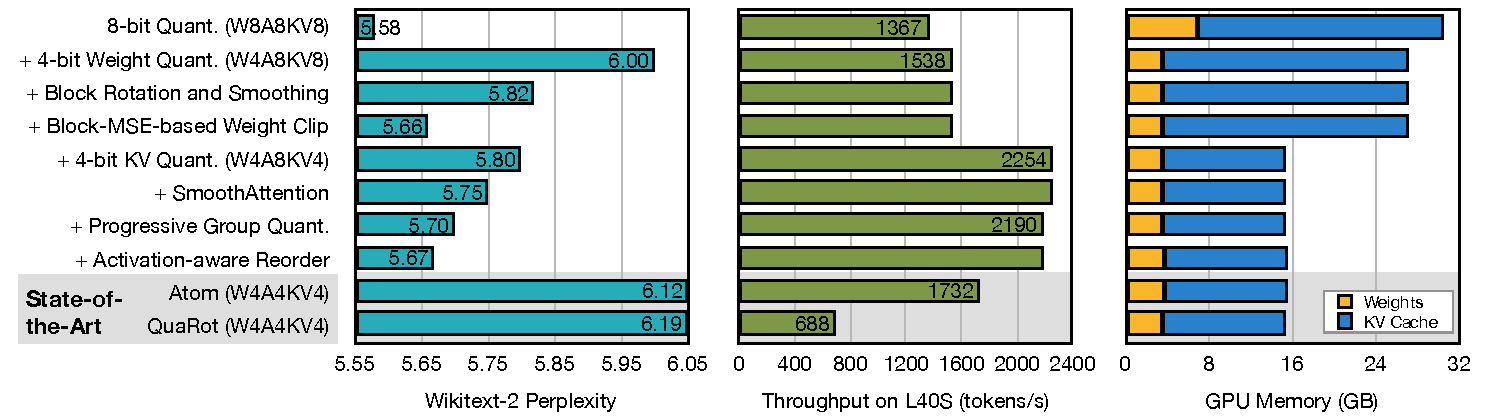
\includegraphics[width=0.95\linewidth]{figure/6-evaluation/algo-ablation-double.pdf}
    \vspace{-10pt}
    \caption{Ablation study on quantization techniques used in \algo and the impact of serving throughput, GPU memory consumption in \system. The model used here is Llama-2-7B.}
    \label{fig:evaluation:alg-ablation}
    \vspace{-10pt}
\end{figure*}


\begin{figure*}[t]
    \vspace{5pt}
    \centering
    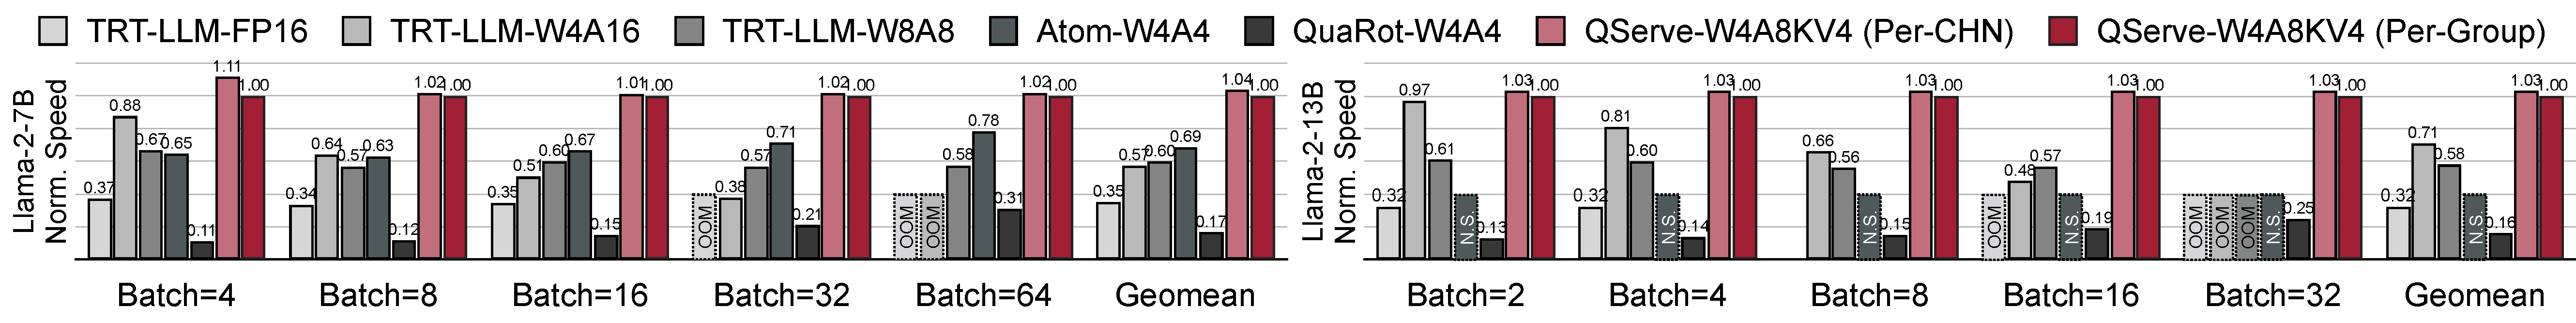
\includegraphics[width=\linewidth]{figure/6-evaluation/speed_same_batch.pdf}
    \vspace{-25pt}
    \caption{Same-batch throughput comparison between \system and baseline systems on L40S. We use an input sequence length of 1024 and output sequence length of 512.} %
    \label{fig:evaluation:main_speed_same_batch}
    \vspace{-5pt}
\end{figure*}







\subsection{Efficiency Evaluation}

We assessed the efficiency of \system on A100-80G-SXM4 and L40S-48G GPUs by comparing it against TensorRT-LLM (using \texttt{FP16}, \textbf{\texttt{W8A8}}, and \textbf{\texttt{W4A16}} precisions), Atom (\textbf{\texttt{W4A4}}), and QuaRot (\textbf{\texttt{W4A4}}). The primary metric for system evaluation is the maximum achievable throughput within the same memory constraints, where we use an input sequence length of 1024 and output sequence length of 512. We notice that Atom only supports Llama-2-7B, and QuaRot does not support GQA. Therefore, we skip these unsupported models when measuring the performance of baseline systems. 

We present relative performance comparisons in Figure \ref{fig:evaluation:main_speed} and absolute throughput values in Table \ref{tab:abs_main_speed}. We use per-channel quantization for A100 and per-group quantization for L40S. This is because L40S has stronger CUDA cores for dequantization. Relative to the best-performing configuration of TensorRT-LLM, \system demonstrates significant improvements on A100: it achieves \textbf{2\x} higher throughput for Llama-1-30B, \textbf{1.2-1.4\x} higher throughput for Llama-2 models, \textbf{1.2\x} higher throughput for Mistral and Yi, and \textbf{2.4\x} higher throughput for Qwen-1.5. The performance improvements are particularly notable on the L40S GPUs, where we observed a throughput improvement ranging from \textbf{1.47\x} to \textbf{3.47\x} across all seven models evaluated. Remarkably, despite the L40S's significantly smaller memory capacity compared to the A100, \system effectively maintains the same batch size as TensorRT-LLM on the A100. This achievement is attributed to our aggressive 4-bit quantization applied to both weights and the KV cache. By examining Table \ref{tab:abs_main_speed}, we clearly observe that serving five of seven models under 34B on L40S with \system achieves even higher throughput than serving them on A100 using TensorRT-LLM. Our performance gain over Atom and QuaRot on A100 is even more prominent since these systems did not outperform TensorRT-LLM. On L40S, \system still achieves 10\% higher throughput than Atom when running Llama-2-7B, the only model supported by their system despite the fact that we use higher quantization precision. Besides, the accuracy achieved by \system is much better than Atom, as indicated in Table \ref{tab:evaluation:zero-shot}.

\subsection{Analysis and Discussion.}

\textbf{Ablation study on quantization techniques.} We examine the impact on accuracy of various quantization techniques implemented in \algo. 
Our analysis begins with round-to-nearest (RTN) \textbf{\texttt{W8A8}} quantization on Llama-2-7B (per-channel + per-token). We then lower the quantization precision and apply different techniques step-by-step. For each step, we evaluated the WikiText2 perplexity and end-to-end inference performance on L40S with 64 requests of 1024 input tokens and 512 output tokens.
The results are detailed in \fig{fig:evaluation:alg-ablation}.
We see that reducing the weight precision to 4 bits significantly impaired the model performance, though it increased end-to-end processing speed by 1.12\x and saved 3.5GB GPU memory. Rotating the block input modules helped suppress the activation outliers, resulting in 0.18 perplexity improvement. In addition, minimizing the block output MSE through weight clipping further decreased the perplexity by 0.16. Consequently, our \textbf{\texttt{W4A8}} configuration has achieved a perplexity comparable to that of \textbf{\texttt{W4A16}}. However, quantizing KV cache to 4 bits again deteriorated model performance by 0.14, although it substantially enhanced the end-to-end inference throughput by 1.47\x and halved GPU memory usage. \smoothattention reduced perplexity by 0.05, without adding system overhead. Progressive group quantization further improved perplexity by an additional 0.04, with only a negligible increase in dequantization overhead. Lastly, activation-aware channel reordering enhanced perplexity by 0.03.


\begin{figure}[t]
    \centering
    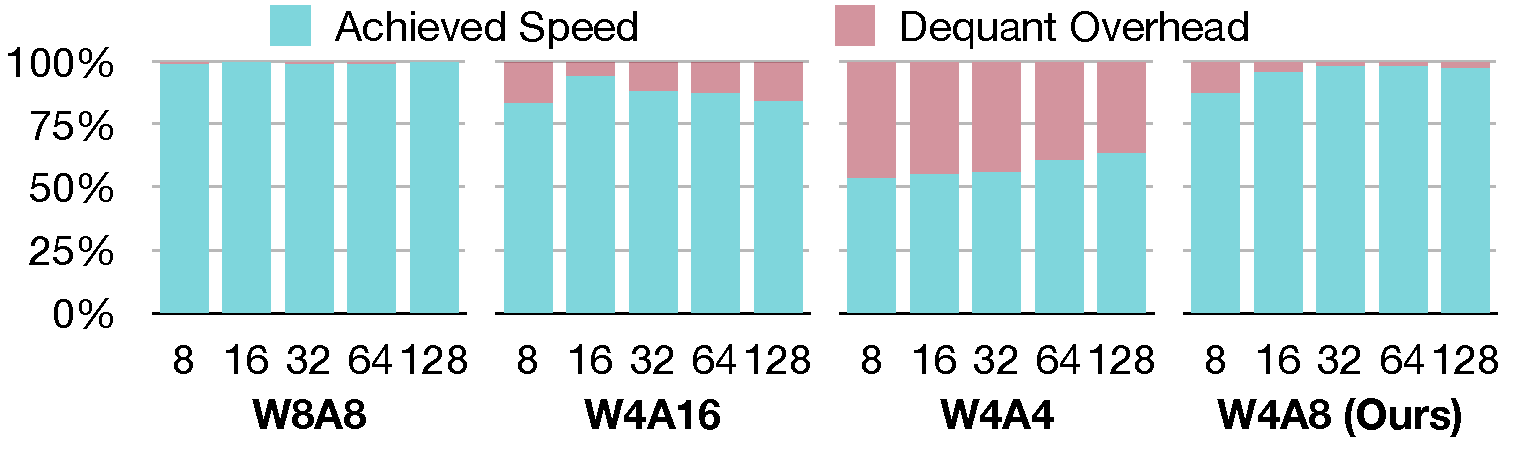
\includegraphics[width=\linewidth]{figure/6-evaluation/dequant_overhead.pdf}
    \vspace{-25pt}
    \caption{The dequantization overhead in \system is much smaller than that in Atom-\textbf{\texttt{W4A4}} (up to 90\%).}
    \label{fig:dequant_overhead}
    \vspace{-20pt}
\end{figure}

\textbf{Ablation study on \system system: Dequantization overhead.} We measure the dequantization overhead of per-group \system-\textbf{\texttt{W4A8}} GEMM and other baselines in Figure \ref{fig:dequant_overhead}. Our dequantization overhead is comparable with TRT-LLM-\textbf{\texttt{W4A16}}, but since we perform computation on \texttt{INT8} tensor cores, we enjoy 2\x higher throughput. 

\textbf{Comparisons under the same batches.} We demonstrate speedup results under the same batch sizes in Figure \ref{fig:evaluation:main_speed_same_batch}. For Llama-2-7B, we show that the 1.88\x speedup over TRT-LLM can be broken down to two parts: 1.45\x from same batch speedup and 1.3\x from the enlarged batch size. For larger models like Llama-2-13B, scaling up the batch size and single batch speedup are equally important (1.7\x improvement). 




\textbf{Improvement breakdown for \texttt{KV4} attention.} We detail the enhancements from attention optimizations in Section \sect{sect:system:attention}. Starting with the basic \texttt{KV4} implementation, which exhibits an A100 latency of 0.48ms for a 64$\times$1024 input, the application of bit tricks from \cite{kim2022says} reduces the kernel latency to 0.44ms. Further improvements are achieved by simplifying the control flow, which reduces latency by an additional 0.05ms. Subsequently, converting the QK and SV products to \texttt{FP16} each contributes a 0.03ms latency reduction. Asynchronous prefetching of dequantization parameters at the start of the attention kernel further enhances performance, ultimately reducing the latency to 0.28ms and achieving an end-to-end improvement of 1.7\x.
